\section{Model}
In this project we will implement the \emph{limited} Texas Hold'em heads-up poker. As we
described in section 2, every hand proceeds in four states pre-flop, folp, 
turn, and river. In each state of a hand, there will be a bidding action 
between agents, then if they concur on the bidding value, the hand will
step into the next state. In the limited poker, the set of all valid actions 
for agents is fold, check, bet two chips. In our model, for each agent
we define two hidden random variables $F$, and $H$, which are not revealed to the
opponent. $F$, is a feature vector representing the agent's properties, \ie her 
level of aggression. $F$ can be quite complicated, to incorporate the 
agent's way of playing in all levels. In our model we only consider one feature 
to represent how much aggressive/conservative the agent is. $H$ is a random
variable representing the agent's hole cards. Note that $H$ is unique for 
each hand of the game and $F$ is unique for each agent.

\subsection{How the agent plays poker?}
The agent will consider two hidden random variables $H$ and $F$ as described above 
for the opponent and tries to update her beliefs about them as she plays. Figure (1) shows the
probabilistic graphical model (PGM) for each state of a 
particular hand that the agent uses to update her 
beliefs. In this model, $B$ represents the dealt cards so far on the board, $S$ is the 
story of the hand so far (\ie the actions in the previous states of the hand), and 
$A$ is the opponent's action. Note that $B$, $S$, and $A$ are all observed by the
agent, and she should use them to update her beliefs about hidden random variable
$H$.
 
\begin{figure}[h!]
  	\centering
 	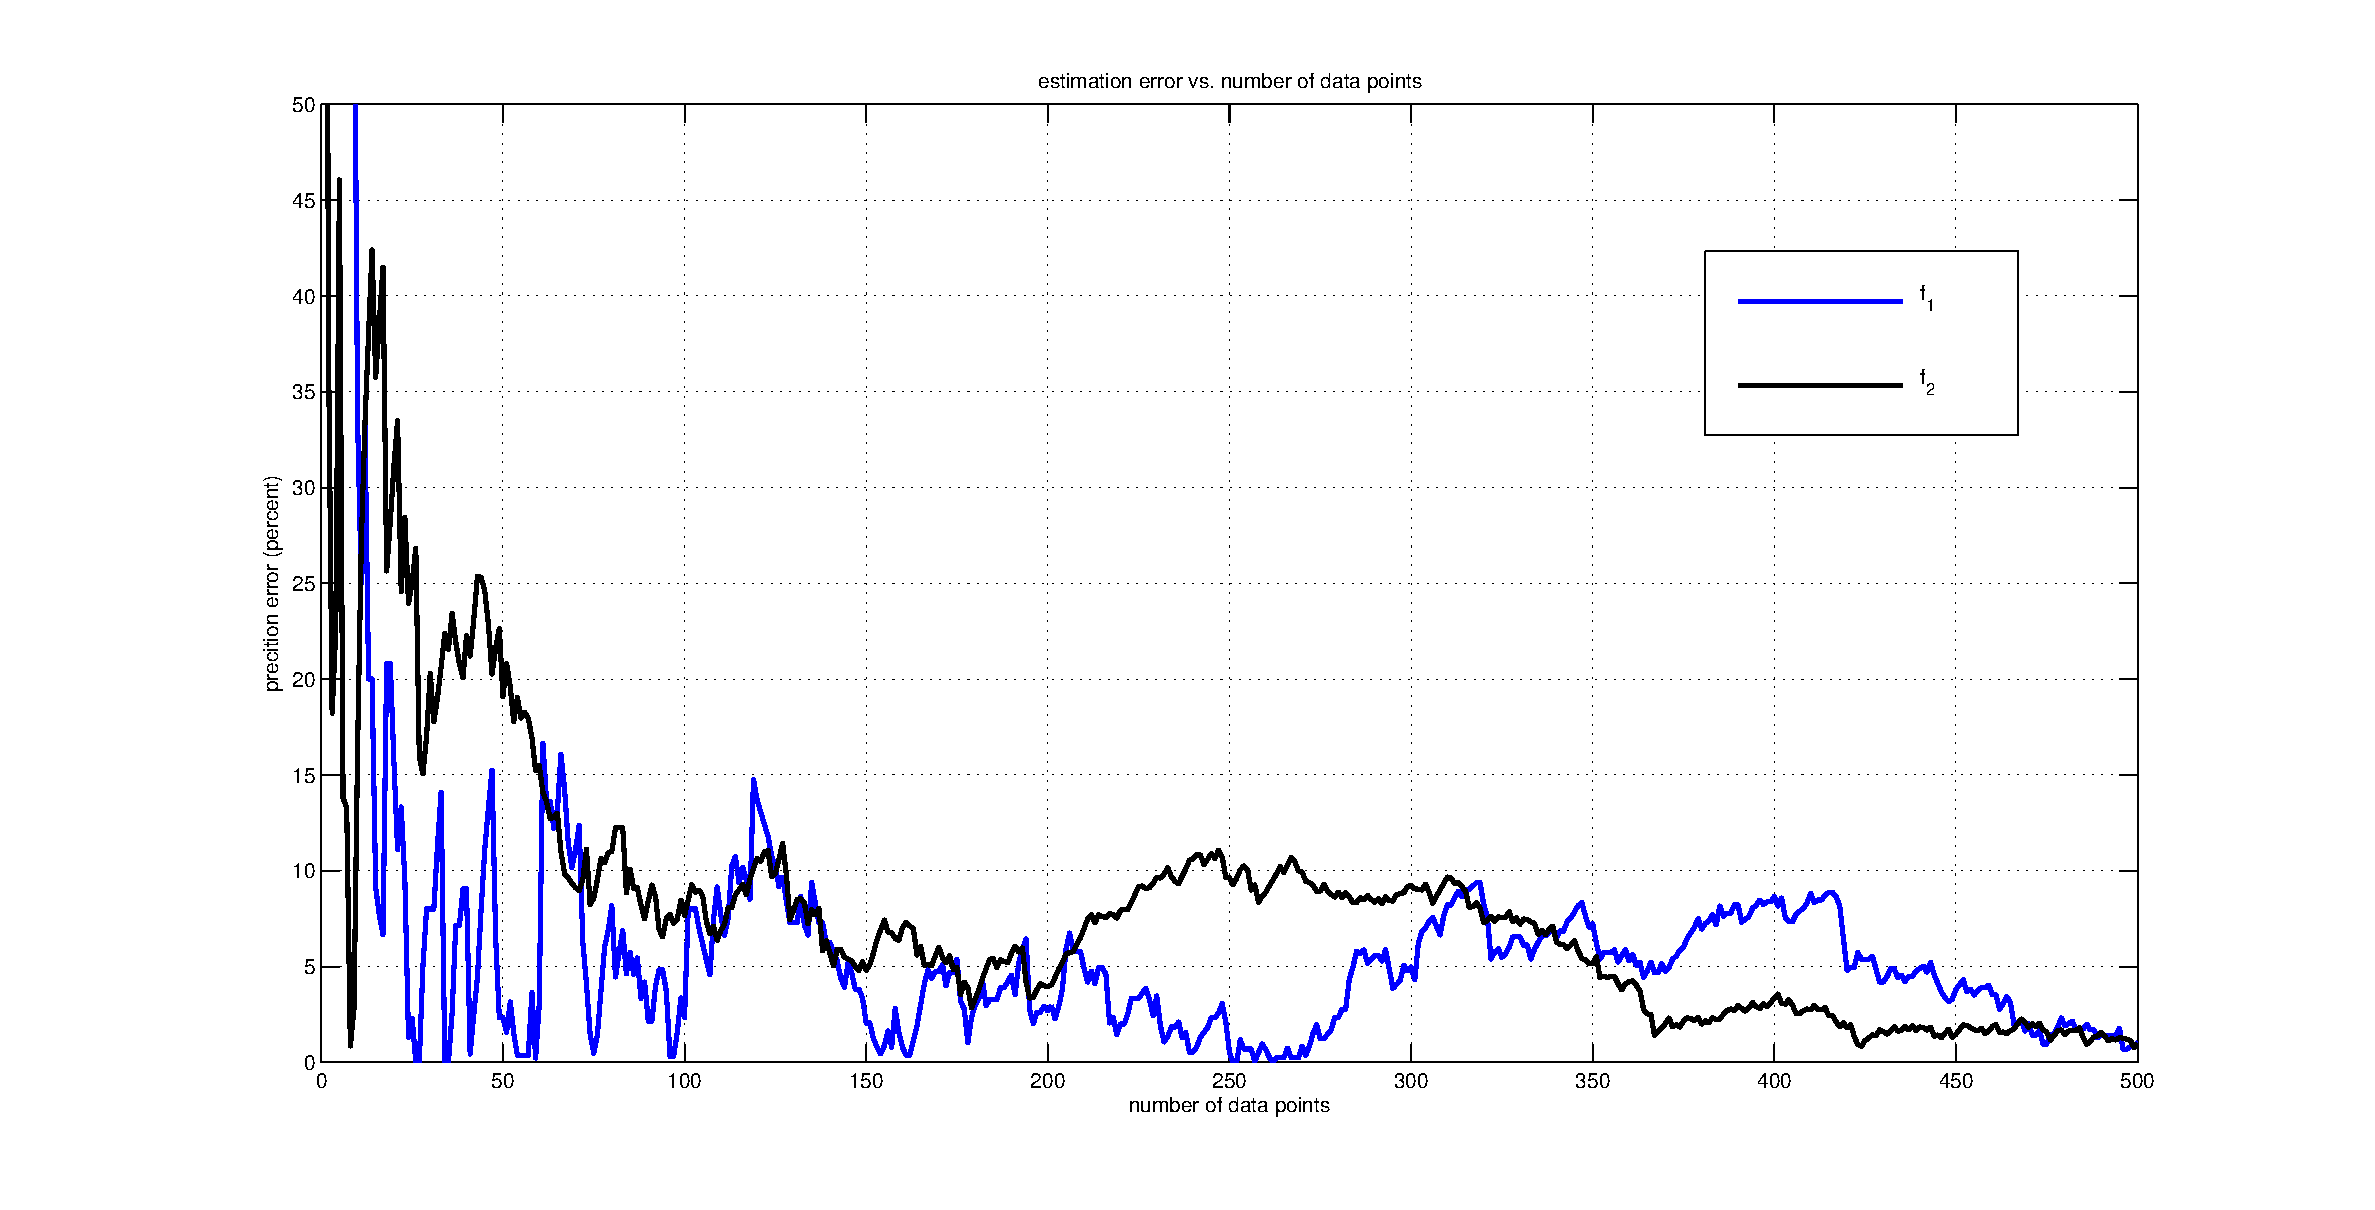
\includegraphics[scale = .55]{fig1}
	\caption{opponent's action PGM}
\end{figure}
